%!TEX root = ../report.tex
\section{Solution}
The paper introduced by van der Laan et al. \cite{van2009screen} provides a fitting solution to our problem.
The paper describes a method for visualizing fluids simulated using SPH in a natural way.
The goal of the paper is to provide a solution to our aforementioned problem.
According to the paper, they want to create:
\begin{enumerate}
	\item \label{en:item1} Achieves real-time performance, with a configurable speed versus quality trade-off.
	\item \label{en:item2} Does all the processing, rendering and shading steps directly on the graphics hardware.
	\item \label{en:item3} Smooths the surface to prevent the fluid from looking blobby or jelly-like.
	\item \label{en:item4} Is not based on polygonization, and thus does not suffer from the associated tessellation artifacts.
\end{enumerate}

Items \ref{en:item1} and \ref{en:item3} have a direct connection with our goals and items \ref{en:item2} and \ref{en:item4} are ways to enable these goals.

The method described in the paper consists of multiple passes. It assumes that there is a functional SPH simulation where each fluid particle has a density. Then each frame the following steps are performed:
\begin{enumerate}
	\item Splat points as spheres and determine depth values per fragment
	\item Smooth the spheres based on curvature flow
	\item Attenuate colors based on thickness
	\item Add noise texture and advect throughout the simulation
	\item Add foam
	\item Render using Fresnel and Phong equations
\end{enumerate}

\subsection{Depth determination}
It is desirable to determine depth of fragment in the simulation in order to know which fragments are part of the surface. 
In order to obtain these depth values, the points from the SPH simulation are splatted to discs and their fragments are subjected to a hardware depth test. 
This result is subsequently written to a depth buffer. 
Note that merely the depth value is splatted and the color and normal attributes are left unchanged as they will be changed in later steps.

\subsection{Surface smoothing}
\label{sec:smoothing}
Smoothing is a critical component in the paper. It is responsible for creating a smooth surface from a set of points so to avoid a blobby and jelly-like surface which is undesirable. The paper argues that this is a better approach than using Gaussian blurring because it performs better and ought to produce better results because there will be no silhouette blurring. 
This is achieved by translating points along the $z$-axis according the curvature flow. 

Curvature flow is defined as the divergence of the normal by \(2H = \nabla \cdot \hat{\mathbf{n}}\). Subsequently, depth values can be displaced every timestep based on the curvature in that point, as \(\frac{\partial z}{\partial t} = H\).

To obtain normals, the point of which the normal needs to be determined is mapped back to a point in view by inverting the projection transformation. This point is called \begin{equation}
	\label{eq:pcalc}
	\mathbf{P}(x, y) = \begin{pmatrix}\frac{\frac{2x}{V_x} - 1.0}{F_x}\\\frac{\frac{2y}{V_y} - 1.0}{F_y}\\1\end{pmatrix}z(x,y) = \begin{pmatrix}W_x\\W_y\\1\end{pmatrix}z(x,y)
\end{equation}
where \(V_x\) and \(V_y\) are the viewport dimensions and \(F_x\) and \(F_y\) is the focal length in \(x\) and \(y\) component.

The normal is then obtained by 
\begin{equation}
	\label{eq:norm}
	\mathbf{n}(x,y) = \frac{\partial \mathbf{P}}{\partial x} \times \frac{\partial \mathbf{P}}{\partial y}
\end{equation}
Rigorous algebra shows that 
\begin{equation}
	\label{eq:normals}
	\mathbf{n}(x,y) = \begin{pmatrix}-C_y\frac{\partial z}{\partial x}\\-C_x\frac{\partial z}{\partial y}\\C_xC_yz\end{pmatrix}z
\end{equation}
Here \(C_x = \frac{2}{V_xF_x}\) and \(C_y = \frac{2}{V_yF_y}\) 

Subsequently, the unit normal must be obtained. This is obtained by \(\hat{\mathbf{n}}(x,y) = \frac{\mathbf{n}(x,y)}{\mid \mathbf{n}(x,y)\mid} = \frac{\mathbf{n}(x,y)}{\sqrt{D}}\) where 
\begin{equation}
	\label{eq:D}
	D = C_y^2 \left(\frac{\partial z}{\partial x}\right)^2 + C_x^2 \left(\frac{\partial z}{\partial y}\right)^2 + C_x^2 C_y^2 z^2
\end{equation}

Now that we have a unit normal we can define mean curvature as 
\begin{equation}
	\label{eq:curvy}
	2H = \frac{\partial \hat{\mathbf{n}}_x}{\partial x} + \frac{\partial\hat{\mathbf{n}}_y}{\partial y} = \frac{C_y E_x + C_x E_y}{D\sqrt{D}}
\end{equation}
in which
\begin{eqnarray}
	E_x &=& \frac{1}{2}\frac{\partial z}{\partial x}\frac{\partial D}{\partial x} - \frac{\partial^2z}{\partial x^2}D\\
	E_y &=& \frac{1}{2}\frac{\partial z}{\partial y}\frac{\partial D}{\partial y} - \frac{\partial^2z}{\partial y^2}D
\end{eqnarray}

These values can be calculated fairly easy and can thus be used to modify the \(z\)-values in the visualization easily and fast using Euler integration in time.

\subsection{Thickness}
The thickness of a fluid is important because an object behind the fluid should change color according to the amount of fluid in front of it.
Also, the thickness is used to determine the transparency and color of the fluid.
This means that the distance from the camera towards the first opaque object has to be determined for each fragment.
Each particle is rendered as a sphere and has a fixed size.
Additive blending is used to determine the total thickness of a surface at each fragment.

\subsection{Noise}
In order to remove the appearance of an artificially smooth surface, noise has to be added.
Since the simulation has moving particles in it, the noise has to advect with those particles for a realistic result.
Also the noise has to have a smaller and larger frequency than the fluid.

Van der Laan \cite{van2009screen} suggests to use Perlin noise \cite{perlin1985image}.
One octave of noise is added to each projected particle, this makes sure that the noise moves along with the fluid flow.
The amount of noise that is added for each particle depends on the depth of the particle with respect to the surface, in other words; noise contributes less as particles submerge.
\begin{equation}
\label{eq:noise}
	I(x,y) = noise(x,y) \ast e^{-x^2 - y^2 - (\mathbf{p}_z(x,y)-d(x,y))^2}
\end{equation}
Equation \ref{eq:noise} shows this noise calculation in a formula.

The noise for every particle is then summed together to get the correct amount of noise per fragment.
Fluids that have a high change in velocity need to be marked, so the noise for that particles is influenced more.
Additive blending is used so the Perlin noise is correctly blended into the fluid.

Also, foam can be added to the fluid by adding grey according to the magnitude of the noise.

\subsection{Rendering}
Finally, all intermediate results are merged together in a final texture that is rendered as full-screen quad.
Since light changes direction when it moves between media, and thus the reflection and refraction vectors changes too, a calculation for this direction change is needed.
A visualization of this behavior can be seen in figure~\ref{fig:fresnel}.
\begin{figure}[!th]
\hrule
\begin{center}
\vspace*{2ex}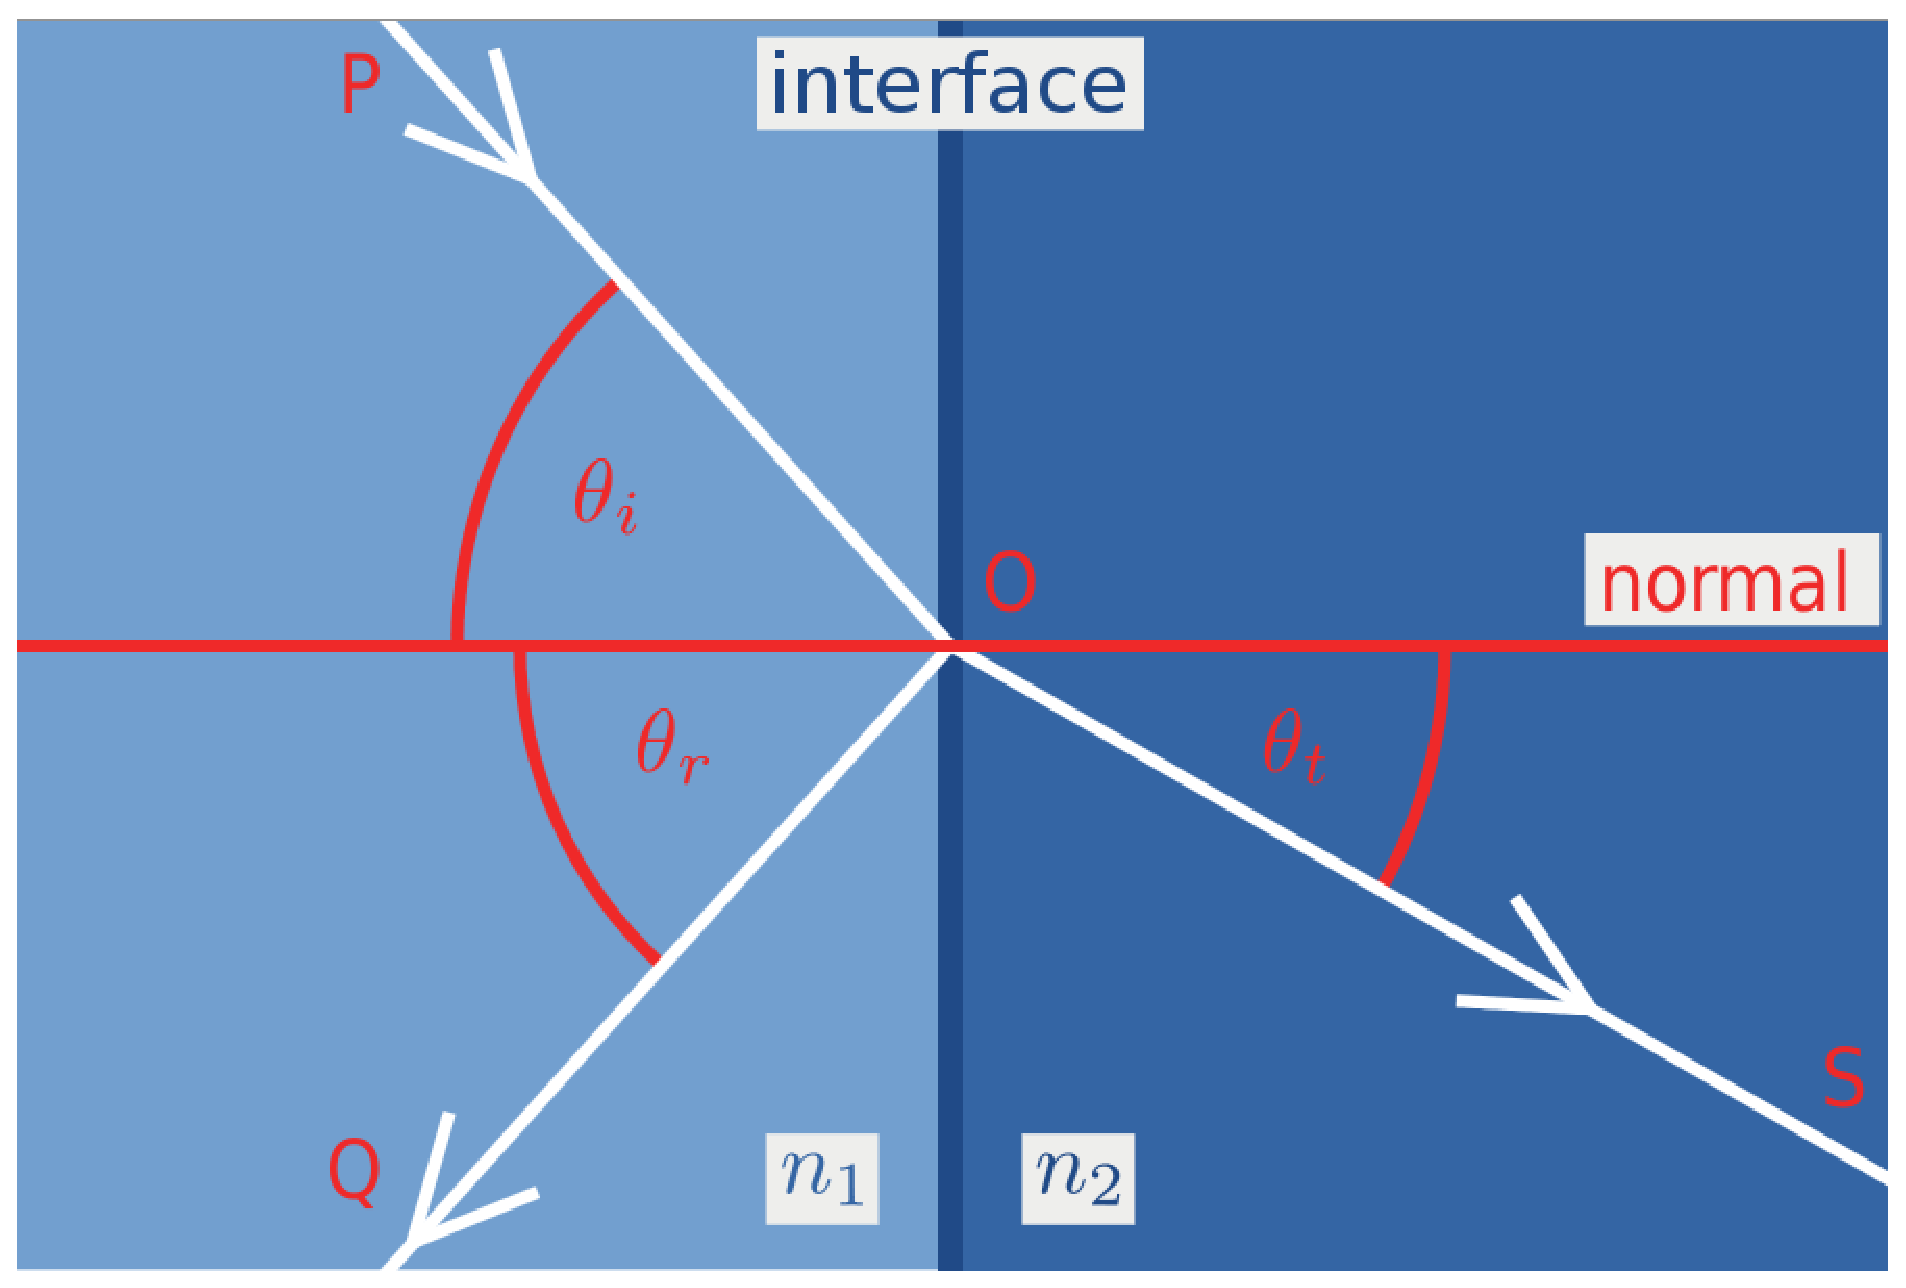
\includegraphics[width=0.48\textwidth]{pictures/Fresnel.eps}
\end{center}
\caption{Light direction change between surfaces (From: \url{http://en.wikipedia.org/wiki/File:Fresnel1.svg})}
\label{fig:fresnel} 
\vspace*{2ex}
\hrule
\end{figure}

The Fresnel equation (by Augustin-Jean Fresnel) is used to calculate the correct reflection and refraction vectors,
\begin{eqnarray}
	R_s &=& \left\vert \frac{n_1 \cos \theta_i - n_2 \cos \theta_t}{n_1 \cos \theta_i + n_2 \cos \theta_t} \right\vert ^2 \\
	T_s &=& 1 - R_s.
\end{eqnarray}
Where $R_s$ is the reflection vector, and $T_s$ is the refraction vector.
The meaning of the other variables can be seen in figure~\ref{fig:fresnel}.
Once these vectors are known, the Phong \cite{phong1975illumination} illumination model can be used for the rendering.

This results in the following equation to determine the output color \cite{van2009screen}:
\begin{equation}
\label{eq:shading}
C_{out} = a(1 - F(\mathbf{n} \cdot \mathbf{v})) + bF(\mathbf{n} \cdot \mathbf{v}) + k_s(\mathbf{n} \cdot \mathbf{h})^\alpha.
\end{equation}
$F$ is the Fresnel equation, $a$ is the refracted fluid color, $b$ is the reflected scene color, $k_s$ and $\alpha$ are both constant and represent the specular highlight. $\mathbf{n}$ is the normal along the surface, $\mathbf{h}$ is the half-angle between the camera and the light, and $\mathbf{v}$ is the direction pointing towards the camera.
